\chapter{引言}\label{chap:introduction}

云计算改变了人们使用计算资源的方式,人们通过云厂商提供的计算服务能够方便地使用到先进硬件资源,同时云计算具备的弹性、安全等特性也能够为人们节省管理负担。近年来,超大规模数据中心在不断增加。2021年统计数据中~\ref{fig:cloud_compute_scale}, 中国的数据中心数量已超700个,而近年来随AI、物联网、区块链与元宇宙等技术的发展,预计将来超大规模数据中心数量仍然会持续增长,在这一背景下,如何利用数据中心丰富的资源,提高数据中心资源利用率成为云厂商关注的核心问题之一。

\begin{figure}[!htbp]
    \centering
    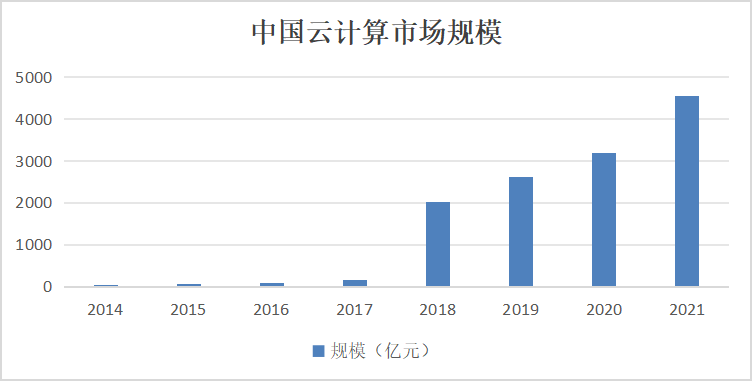
\includegraphics[width=0.40\textwidth]{cloud_compute_scale}
    \bicaption{\quad 中国云计算市场规模增长趋势}{\quad cloud_compute_scale}
    \label{fig:cloud_compute_scale}
\end{figure}

资源超卖是云厂商提高数据中心资源利用率、增加收入的主要手段之一。超卖主要涉及计算资源与存储资源。CPU是最常见的超卖资源,虚拟化技术允许在一个CPU运行多个虚拟CPU,超卖意味着售出的虚拟CPU资源超过了当前节点上物理核心数量,内存超卖则依赖内存页共享交换机制,但不同于CPU资源超卖,内存的超卖风险较高,因为一旦物理内存耗尽,就会导致系统性能的急剧下降,存储超卖则意味着出售给用户比节点实际存储还要多的存储资源,这通常基于用户一般不会完全使用存储空间的假设,而存储池的设计也能够及时的满足用户的存储需求,网络带宽同样可以进行超卖,这是因为用户在网络的使用存在时间上的不均,同时也依赖一定的网络调控手段来避免网络出现拥塞和劣化。

随虚拟化技术不断进步,从以Xen、KVM技术为核心的虚拟机,到以容器为核心的kubernetes,再到更前沿的ServerLess、FaaS平台,虚拟化技术的提升对用户屏蔽了越来越多的底层细节,使得用户能够越来越专注核心的业务逻辑,而对云厂商而言,则能够提供更细粒度的计算、存储资源。

\begin{figure}[!htbp]
    \centering
    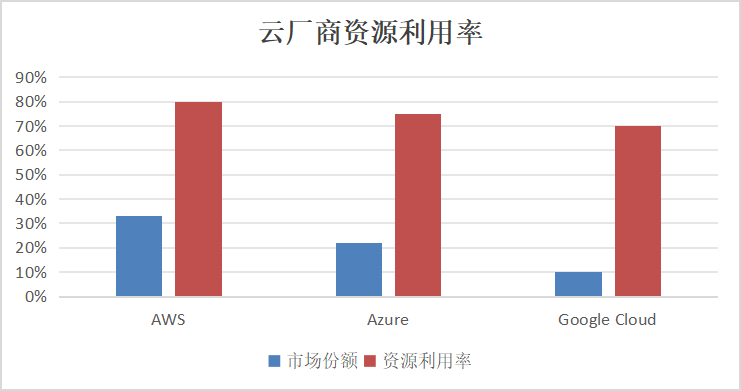
\includegraphics[width=0.40\textwidth]{cloud_compute_utilization}
    \bicaption{\quad 云厂商市场份额及利用率}{\quad cloud_compute_utilization}
    \label{fig:cloud_compute_utilization}
\end{figure}

细粒度的资源管理意味着更多的超卖机会,然而不恰当的超卖策略会对用户产生较严重影响,同时越上层的虚拟化技术能够提供给用户的信息越少,导致用户难以通过常规的手段去观测或调优。但是如同商品需要提供质量凭证,云厂商也应当为其所出售的云产品提供质量保证,因此云厂商会与用户协商云产品的SLO,用来指定来指定云产品所提供功能的一种期望状态,通常包含每秒请求数量、延迟、服务可用性以及带宽等关键性能指标,并协商在违反SLO是对用户予以补偿。

SLO为用户提供了保证,也意味着SLO的破坏会给用户及云厂商都带来损失,在提升资源利用率与SLO保证中取舍是云厂商需要关注的核心问题之一。实现SLO保证依赖持续的监测与调度机制。可观测性技术是常见的监控机制,其通常为一套数据采集系统,从应用内、运行时及集群获取不同纬度的监控信息,帮助运维人员了解云产品的运行情况。应用内的可观测性机制通常为内嵌的性能监控代码,在应用运行时记录性能信息,并提供API接口以便外部访问,这些指标能够直接反映SLO。运行时的可观测性则从应用运行的上下文中获取有效信息,如内核中对任务使用资源的统计。集群可观测性突出多节点的特征,反映端到端的性能情况,在微服务背景下,集群级别的可观测性机制越来越重要。可观测性系统除实时监控以外,还可包括数据的存储、查询的部分,而通过对离线数据的建模分析,进而能够对SLO预测,以便更早地定位SLO破坏。调度机制可分为面向任务与面向资源的调度。面向任务的调度前提是系统中存在不同的隔离域,然后基于域内的资源使用情况决定任务放置的位置。kubernetes集群中不同的节点就是不同隔离域,每个节点有不同的资源使用情况,kubernetes提供了一套灵活的标签机制来对各个节点的资源进行描述,scheduler是kubernetes中负载调度的组件,其在运行时监听Pod的创建请求并依据标签及可编程的调度逻辑匹配合适的节点,完成Pod的调度。而在节点侧进行任务调度的通常是操作系统,Linux中会维护每个CPU的负载水平,当有一个新的进程执行时,就会依据CPU的繁忙程度进行放置,同时系统在长时间的运行过程中进程会不断变化,因此Linux还会通过工作窃取等方式对各个CPU进行负载均衡。面向资源调度考虑应用通常在资源不足时发生性能劣化,因此采用调整资源分配的方式来进行调度。分时复用构造了时间上的隔离域,Linux可以通过增加进程的可用时间片数量,让进程使用更多的CPU资源,CAT[1]技术则允许对进程的LLC、内存带宽资源进行划分,从而能够让进程出让相关资源,缓解系统中的资源争用情况。

SLO保障机制在集群与节点两种维度有不同的实施方案。其中集群维度发展迅速,随容器、kubernetes技术的不断迭代,云原生理念得到更广泛的推广,越来越多的应用以容器的形式部署到云平台中,容器本身仍然是进程,因此不存在类似虚拟机的信息墙,这些都为开发者提供了便利,围绕容器的云原生可观测性技术已经发展出相当丰富的生态。kubernetes是集群管理的核心,采用微服务的架构,由多个相互解耦的组件构成,其中scheduler是调度的核心组件,kubernetes提供了丰富的接口供开发者定制。集群纬度丰富的可观测性生态与调度可定制性,使得SLO保障机制够较为方便地进行设计、部署及效果验证。节点维度也有丰富的可观测性与调度手段,但由于较长发展时间所产生的复杂软件环境,当前并没有相对统一观测与调度机制,通常需要引入其他手段同步各参差的信息,因此产生的的短板效应会带来较高的调度延迟与误差,实践中节点纬度的保障机制通常围绕内核展开,而内核默认提供的CFS调度策略并不能满足云厂商对保障SLO的需求,但修改调度器通常较复杂,且部署调度策略时需要中断内核的执行,会引入额外的运维风险,基于以上种种原因,节点维度的相关研究实践开展缓慢。

但节点维度相较于集群维度有不可替代的优势。首先在调度延迟上,集群维度中各个组件的相互通信依赖节点间网络通信,信息的编解码、传输都会带来一定的延时,这导致集群维度的监控与调度通常都采用较粗的时间粒度,而在网络流量突发的场景则容易遗漏或是产生乒乓效应。而节点维度则不同,由于更靠近设备,因此能够更快速的监测硬件状况,并且内核通常都以us时间粒度进行调度决策,这说明节点维度更适合进行细粒度的监测及调度,更细的粒度也就意味着更多的超卖机会,而节点维度的效果提升能够借助集群的规模化效应进一步扩大,因此节点维度尽管困难,但对于云厂商而言仍然十分重要。

\begin{figure}[!htbp]
    \centering
    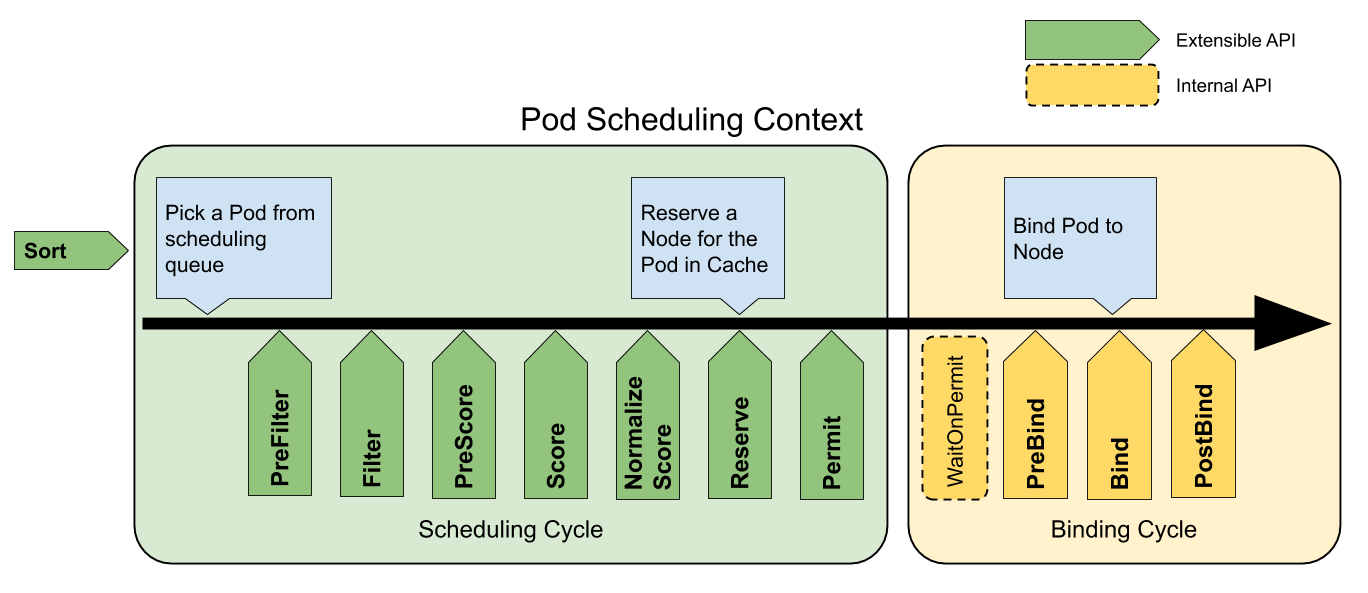
\includegraphics[width=0.40\textwidth]{k8s_scheduler}
    \bicaption{\quad k8s调度流程}{\quad k8s_scheduler}
    \label{fig:k8s_scheduler}
\end{figure}

kubernetes基于标签的调度机制流程如图所示~\ref{fig:k8s_scheduler},其极强的灵活性有助于开发者应对不同应用的不同资源需求。但在节点侧,调度机制因其设计上的不灵活,往往阻碍了节点侧SLO保障机制发展。节点侧通常提供有限的调度手段,如将CPU敏感度作为标签,则nice值能够很好地实现此标签的功能,更低的nice值意味着应用能够分配到更多的时间片,从满足应用对CPU资源的需求。然而当前数据中心中应用多样,分析云场景中常见应用的监测数据,发现这些应用在资源的使用上存在较大差异,单一资源的调控难以满足节点侧调度的需求。为解决开发者的需求,内核引入了Cgroup技术,允许在CPU、Memory、Network、IO等各个子系统中细粒度的资源上调控,每一个Cgroup都可以视为一种标签,在内核的发展过程中,Cgroup与调度子系统的结合也越来越紧密。本论文希望在节点维度提供一种基于标签的节点侧调度机制,并借助节点侧在时间、资源粒度上的优势,提供更好的SLO保障。

\section{本文的研究背景与意义}

\section{国内外相关研究}

\section{论文的研究内容}

\section{论文结构安排}
